\section{Evaluating Operational Networks with \rcc}\label{sec:evaluation}

Our goal is to help operators move away from today's mode of
stimulus-response reasoning by allowing them to check the correctness of
their configurations {\em before} deploying them on a live network.
\rcc has helped network operators find faults in deployed
configurations; we present these findings in this section.  Because we
used \rcc 
to test configurations that were {\em already deployed} in live
networks, we did not expect \rcc to find many of the types of transient
misconfigurations that Mahajan {\em et al.} found~\cite{Mahajan2002}
(\ie, those that quickly become apparent to operators when the
configuration is deployed).  If \rcc were applied to BGP configurations
before deployment, we expect that it could prevent more than 75\%
of the ``origin misconfiguration'' incidents and more than 90\% of the
``export misconfiguration'' incidents described in that
study.\footnote{\rcc detects the following classes of
  misconfiguration described by Mahajan {\em et al.}: reliance on
  upstream filtering, old configuration, community,
  forgotten filter, prefix-based config, bad ACL or route map, and typo.}

\subsection{Analyzing Real-World Configurations}

We made \rcc
available to operators, hoping that they would run it on their
configurations and report their results.
As a result, we were able to use \rcc to evaluate the configurations
from 17 real-world networks, 
including BGP configurations from every router in 12 ASes.  

Network operators are reluctant
to share router configuration because it often encodes
proprietary information.
Also, many ISPs do not like researchers reporting on mistakes in
their networks.  (Previous efforts have enjoyed only limited success
in gaining access to real-world
configurations~\cite{www-uw-configdonate}.)  
We learned that  providing operators with a useful tool or service
increases the likelihood of cooperation.
When presented
with \rccns, many operators opted to provide us with configurations,
while others ran \rcc on their configurations and sent us the 
output.

\rcc detected over
1,000 configuration faults.  The size of these networks ranged from two
routers to more than 500 routers. 
Many operators insisted that the details of their configurations be kept
private, so we cannot report separate statistics for each network that
we tested.  Every network we tested had BGP configuration
faults, and operators were
usually unaware of the faults in their networks.
%, which confirms our
%hypothesis that 
%many configuration faults are not apparent.


%% Getting configs is hard.  People protect their configs like their
%% firstborns.  Getting access to configs is an act of faith; building up
%% trust/relationships in operator community help immensely. (Already
%% having these relationships helps even more.)  Still, operators are
%% unlikely to cough up configuration files.  
%% While the tool elicited a relatively small response from the operator
%% community (roughly 30 operators---only a small fraction of network
%% operators---downloaded \rcc, and considerably fewer actually bothered to
%% install and run it), having a configuration checking tool already
%% written before we asked for configuration files made operators more
%% willing to give us network configurations to test their networks.  We
%% also discovered that router vendors can be a good source of BGP
%% configurations; many of these vendors have BGP configurations from parts
%% of their customers' networks.



%% In other
%% cases, \rcc detected configuration anomalies that were not in fact
%% errors, merely the fruits of operator creativity.  We present some of
%% the more interesting examples we discovered in real-world configuration
%% in Section~\ref{sec:anecdotes}.
%\subsection{BGP Configuration Errors and Anomalies}
%% In this section, we some configuration errors that we found particularly
%% interesting or surprising.  Additionally, our experience with analyzing
%% a wide variety of BGP configurations allowed us not only to discover the
%% types of errors that appear in practice, but also to find subtle
%% differences in vendors' BGP implementations and creative configuration
%% tricks that network operators use to accomplish various tasks.


%% Do NOT EDIT BY HAND!  Generated Automatically w/perl.
\begin{table}[t]
\begin{center}

{\footnotesize
\vspace*{-0.1in}
\begin{tabular}{@{}p{2.25in}|rr@{}}
{\bf Problem} & {\bf Latent} & {\bf Benign} \\ \hline  \hline
\multicolumn{3}{@{}c@{}}{{\it Path Visibility}} \\ \hline
{\bf Dissemination Problems} \\
%%
Signaling partition: \\
\hspace*{0.1in} - of route reflectors & 4 & 1 \\
\hspace*{0.1in} - within a RR ``cluster'' & 2 & 0 \\
\hspace*{0.1in} - in a ``full mesh'' & 2 & 0 \\
%%
Routers with duplicate: \\
\hspace*{0.1in} - loopback address & 13 & 120\\ 
%%\hspace*{0.1in} - cluster ID &  &  \\
iBGP configured on one end & 420 & 0 \\  
   or not to loopback &  &  \\  
%%synchronization enabled & 10 & 0 \\

\hline  \hline
\multicolumn{3}{@{}c@{}}{{\it Route Validity}} \\ \hline
{\bf Filtering Problems} \\
transit between peers  & 3 & 3 \\
inconsistent export to peer & 231 & 2 \\
inconsistent import & 105 & 12 \\ 

eBGP session: \\
\hspace*{0.1in} - w/no filters & 21 & --- \\ 
\hspace*{0.1in} - w/undef. filter & 27 & --- \\
\hspace*{0.1in} - w/undef. policy & 2 & --- \\
filter: \\
\hspace*{0.1in} - w/missing prefix & 196 & --- \\
policy: \\
\hspace*{0.1in} - w/undef. AS path & 31 & --- \\
\hspace*{0.1in} - w/undef. community & 12 & --- \\
\hspace*{0.1in} - w/undef. filter & 18 & --- \\



\hdashline[1pt/1pt]
{\bf Dissemination Problems} \\
prepending with bogus AS & 0 & 1 \\
originating unroutable dest. & 22 & 2 \\ 
incorrect next-hop & 0 & 2 \\

\hline \hline
\multicolumn{3}{@{}c@{}}{{\it Determinism}} \\ \hline

{\bf Ranking Problems} \\
nondeterministic MED & 43 & 0 \\
age-based tiebreaking & 259 & 0 \\



\end{tabular}
}
\caption{BGP configuration faults in 17 ASes.} 
\label{tab:errors}
\end{center}
\end{table}


%We classified actual configuration mistakes as errors and cases where
%an operator told us that 
%the ``error'' was a special case as anomalies.
%(Because operators can configure BGP in many ways, \rcc
%sometimes incorrectly flagged errors that were
%configuration ``tricks''.)

\subsection{Fault Classification and Summary}

Table~\ref{tab:errors} summarizes the faults that \rcc detected.
\rcc discovered potentially serious configuration faults as
well as benign ones.  The fact that \rcc discovers benign faults
underscores the difficulty in specifying correct behavior.  
Faults
have various dimensions and levels of seriousness.  For example, one
iBGP partition indicates that \rcc found 
one case where a {\em network} was partitioned, but one instance of
unintentional transit means that \rcc found two {\em sessions} that,
together, caused the AS
to carry traffic in violation of high-level policy.
The absolute number
of faults is less important than noting that many of the faults occurred
at least once.  

Figure~\ref{fig:err_by_as} shows that many faults appeared in many
different ASes.  
We did not observe any significant correlation between
network complexity and prevalence of faults, but configurations from
more ASes are needed to draw any strong conclusions.  The rest of this
section describes the extent of the configuration faults that we found
with \rccns.  We survey faults related to path visibility, route
validity, and determinism, respectively.


%Second, the errors vary in seriousness; one iBGP
%signaling partition is more serious than a handful of incomplete iBGP
%sessions that don't create any partitions.  We classify
%errors according to three levels of seriousness.

%We also shed light on {\em why} we think these errors are
%occurring and recommend possible changes to the protocol and
%configuration languages to reduce the likelihood of these errors.


\subsection{Path Visibility Faults}

The path visibility faults that \rcc detected involve iBGP signaling and
fall into three categories: 
problems with ``full mesh'' and route reflector configuration, problems
configuring route reflector clusters, and incomplete iBGP session
configuration.  Detecting these faults required access to
the BGP configuration for every router in the AS.  



{\bf iBGP signaling partitions.}  
%Every network configuration we
%checked with \rcc that used route reflection had at least one signaling
%partition.  
iBGP signaling partitions appeared in one of two ways: (1)~the top layer
of iBGP routers was not a full mesh; or (2)~a route reflector cluster had
two or more route reflectors, but at least one client in the cluster did
not have an iBGP session with every route reflector in the cluster.
Together, these accounted for $9$ iBGP signaling partitions in 5
distinct ASes, one of which was benign. While most 
partitions involved route reflection, we were surprised to find that
even small networks had iBGP signaling partitions.  In one network of
only three routers, the operator had failed to configure a full mesh; he
told us that he had ``inadvertently removed an iBGP session''.
\rcc also 
found two cases where routers in a cluster with multiple route
reflectors did not have iBGP sessions to all route reflectors in that
cluster.

\rcc discovered one benign iBGP signaling partition.  The AS in question
had a
group of routers that did not exchange routes with the rest of the
iBGP-speaking routers, but the routers that were partitioned introduced
all 
of the routes that they learned from neighboring ASes into the IGP,
rather than readvertising them via iBGP.  The operator of this network
told us that these routers were for voice over IP (VoIP) traffic; presumably,
these routers injected all routes for this application into the IGP to
achieve fast convergence after a failure or routing change.  
In cases such as these, BGP configuration cannot be checked in isolation
from other routing protocols.

\begin{figure}[t!]
\centering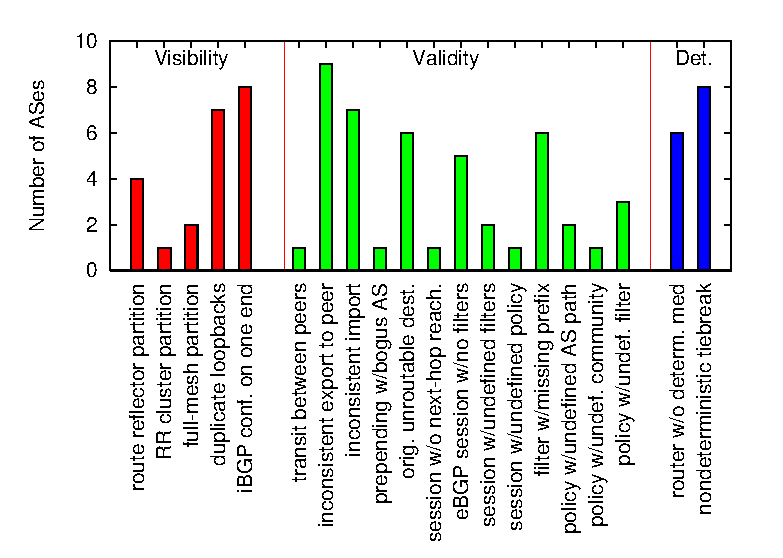
\epsfig{file=rcc/figures/errors_by_as_thesis.eps, width=0.9\linewidth}
\caption{Number of ASes in which each type of fault occurred
  at least once.  
%Unless noted in parentheses, each test was run on all
%  17 ASes.
} 
\label{fig:err_by_as}
\end{figure}



%This example underscores the flexibility
%that operators have in configuring routing protocols and, thus, why
%defining hard and fast correctness rules for BGP is extraordinarily
%difficult.

%% iBGP's goal is simple, but its mechanisms are so complex and obscure
%% that making 
%% mistakes is easy.  We are still discovering
%% configuration subtleties that 
%% fundamentally affect iBGP's correctness.  A replacement for iBGP
%% would eliminate most of these problems.

{\bf Route reflector cluster problems.}  In an iBGP
configuration with route reflection, multiple route reflectors may serve
the same set of clients.  This group of route reflectors and its clients
is called a ``cluster''; each cluster should have a unique ID, and all
routers in the cluster should be assigned the same cluster ID.  If a
router's BGP configuration does not specify a cluster ID, then typically
a router's loopback address is used as the cluster ID.  If two routers
have the same loopback address, then one router may discard a route
learned from the other, thinking that the route is one that it had
announced itself.  \rcc found $13$ instances of routers in distinct clusters
with duplicate loopback addresses and no assigned cluster ID.
%(Table~\ref{tab:errors} shows all cases of duplicate loopback
%addresses, most of which were benign).  
Often, these apparent mistakes may be benign: different physical routers
in the same AS may legitimately have identical loopback addresses.  For
example, routers in distinct IP-layer virtual private networks may route
the same IPv4 address space.


{\bf Incomplete iBGP sessions.} \rcc discovered 420 incomplete iBGP
sessions (\ie, 
a configuration statement on one router indicated the presence of an
iBGP session to another router, but the other router did not have an
iBGP session in the reverse direction).  Many of these faults are likely
benign.  The most likely explanation for the large number of
these faults is that network operators may disable sessions by removing the
configuration from one end of the session without ever ``cleaning up''
the other end of the session.


%\rccns's tests for path visibility in operational networks allowed us to
%discover the following:
%\begin{enumerate}
%\itemsep=-1pt
%\item iBGP configuration is not easy: networks that implemented iBGP
%  with route reflection often had signaling partitions, but \rcc even
%  discovered a small network that had not correctly configured ``full
%  mesh'' iBGP.
%\item Routers occasionally distribute all eBGP-learned routes via IGP,
%  rather than iBGP; in these cases, the fact that a router does not
%  communicate with other routers via iBGP does not matter.
%\item Some aspects of BGP configuration are not maintained or
%  updated as network configuration changes: many configuration files had
%  ``code fragments'' that were vestiges of old BGP sessions but served
%  no function.
%\end{enumerate}

%\rcc also found many instances
%where hundreds of lines of router configuration had been decommissioned.
%In some cases, iBGP sessions (or parts of iBGP sessions) were
%``shutdown'' but remained in the router configuration files.  
%\rcc can
%help operators clean configuration files by highlighting these latent
%faults. 

%%\subsubsection{Route Installation Problems}

%% {\bf Synchronization.}  
%% %Because most ASes only have routers that
%% %participate in iBGP, the configuration option that requires iBGP to be
%% %``synchronized'' with the IGP~(Section~\ref{sec:vis_install}) is usually
%% %disabled.  
%% %Several router vendors disable this option entirely (although
%% %one major vendor still enables the option by default for no good
%% %reason).  
%% We discovered three routers that enabled synchronization; we were unable
%% to contact the operator to find out why 
%% (a vendor provided us with anonymized
%% configurations of one if its customers), but they appeared to be
%% mistakes.  The vendor speculated that their automatic configuration
%% tool may at one time have been configured to enable synchronization by
%% default.

%\item dangling sessions.  things that were established for a specific
%  purpose (\eg, an IETF meeting) and never dismantled afterwards.
%\item duplicate sessions: one to a loopback, one to an interface.
%\item duplicate loopback addresses (\ie, on two different routers)
%\item failure to restore the iBGP mesh after experimentation (ILAN)

%\begin{itemize}
%\itemsep=-1pt
%\item send-community off
%\end{itemize}

%\subsubsection{Anomalies and Curiosities}\label{sec:anomalies}
%Anecdotal stuff.  probably can include stuff here regarding some of the
%  conversations I had with jrex + some ``common nanog knowledge''.  for
%  example,



%interesting
%%  info-flow-control. talk about the DP2AOL community being used to allow
%%  two ``peers'' to use a third ISP for transit.  (note yet
%%  another reason why operators like to keep their configs private)


\subsection{Route Validity Faults}

In this section, we discuss route validity faults.  We first discuss
filtering-related faults; we classify faults as latent unless
a network 
operator explicitly told us that the fault was benign.  
We also describe faults concerning undefined references
to policies and filters.  Some of these faults, while simple to check,
could have serious consequences (\eg, leaked routes), if \rcc had not
caught them and they had been activated.
Finally, we present
some interesting route validity faults related to route dissemination,
all of which 
were benign.  


\subsubsection{Filtering Problems}

Decomposing policies across configurations on different routers can
cause faults, even for relatively simple policies.  \rcc discovered the
following problems: 


{\bf Transit between peers.}  \rcc discovered three instances where
routes learned from one peer or provider could be readvertised to
another; typically, these faults occurred because an export policy for a
session was intended to filter routes that had a certain community
value, but the export policy instead referenced an undefined community.

Obsolete contractual arrangements can remain in configuration long after
those arrangements expire.  \rcc discovered one AS that appeared to
readvertise certain prefixes from one peer to another.  Upon further
investigation, we learned that the AS was actually a previous owner of
one of the peers.  When we notified the operator that his AS was
providing transit between these two peers, he told us, ``Historically,
we had a relationship between them.  I don't know what the status of that
relationship is these days.  Perhaps it is still active---at least in
the configs!''


{\bf Inconsistent export to peer.}  We found $231$ cases where an
AS advertised routes that were not ``equally good'' at every peering
point.  It is hard to say whether these inconsistencies are benign
without knowing the operator's intent, but roughly twenty of these
inconsistencies were certainly accidental. For example, one
inconsistency existed because of an undefined AS path regular expression
referenced in the export policy; these types of inconsistencies have
also been observed in previous measurement studies~\cite{Feamster2004b}.


{\bf Inconsistent import policies.} A recent measurement study observed
that ASes often implement policies that result in late exit (or ``cold
potato'') routing, where a router does not select the BGP route that provides
the closest exit point from its own
network~\cite{Spring2003}.\footnote{Inconsistent import policy technically
  concerns how configuration affects {\em ranking}, and it is more
  often intentional than not.  Nevertheless, this test occasionally highlights
  anomalies that operators are interested in correcting, and it serves
  as a useful sanity check when looking for other types of anomalies (such as
  dynamically detecting inconsistent route advertisements from a
  neighboring AS~\cite{Feamster2004b}).}   \rcc 
found $117$ instances where an AS's import policies explicitly
implemented cold potato routing, which supports this previous
observation.  In one network, \rcc detected a different import policy
for {\em every} session to each neighboring AS. In this case, the import
policy was labeling routes according to the router at which the route
was learned. 

Inconsistent import and export policies were not always
immediately apparent to us upon casual inspection, even after \rcc
detected them. In one case, two 
sessions applied policies with the same name, and both policies were
defined with verbatim configuration fragments.  The difference
resulted from the fact that the difference in policies was three levels
of indirection deep.  For example, one inconsistency occurred because of
a difference in the definition for an AS path regular expression that
the export policy referenced (which, in turn, was referenced by the
session parameters).



%\begin{enumerate}
%\itemsep=-1pt
%% \item BGP configuration often does not follow best common
%%   practices (\eg, filters that reject routes for private or unallocated
%%   prefixes, and deterministic route selection) if the failure to do so
%%   has not yet caused a problem.
%\end{enumerate}

\rcc also detected filtering problems on
single-router configurations:

{\bf Undefined references in policy definitions.} Several large networks
had router configurations that 
referenced undefined variables and BGP sessions that referenced
undefined filters.  
These faults can sometimes result in
unintentional transit or inconsistent export to peers or even potential
invalid route advertisements. 
In one network, \rcc found four routers with undefined filters that
would have allowed a large ISP to accept and readvertise {\em any} route to
the rest of the Internet (such a failure actually occurred in
1997~\cite{www-as7007}, as we described in Section~\ref{sec:intro:problem});
this potentially active fault could have been  
catastrophic if 
a customer had (unintentionally or intentionally) announced invalid routes,
since ASes typically do not filter routes coming from large ISPs.  This
misconfiguration occurred even though the router
configurations were being written with scripts; an operator had
apparently made a mistake specifying {\em inputs} to the scripts.
%These problems mostly seem to surface in configurations where
%operators said they were frequently changing settings.


{\bf Non-existent or inadequate filtering.}  
%As we described in
%Section~\ref{sec:val_filters}, correct filtering practices do not
%guarantee validity, but they certainly prevent obviously invalid routes
%from propagating.  Missing or incorrect import filters can result in
%invalid routes being propagated within an AS and advertised to other
%ASes.  
Filtering can go wrong in several ways: (1)~no filters are used
whatsoever, (2)~a filter is specified but not defined, or
(3)~filters are defined but are missing prefixes or otherwise
out-of-date (\ie, they are not current 
with respect to the list of private and unallocated IP address
space~\cite{www-cymru-bogon}). 

Every network that \rcc analyzed had faults in filter configuration.
Some of these faults would have caused an AS to readvertise {\em any}
route learned from a neighboring AS.  In one case, policy
misconfiguration caused an AS to transit traffic between two of its
peers.  Table~\ref{tab:errors} and Figure~\ref{fig:err_by_as} show that
these faults were extremely common: \rcc found 21 eBGP sessions in 5
distinct ASes with no filters whatsoever and 27 eBGP sessions in 2 ASes
that referenced undefined filters.  Every AS had partially incorrect
filter configuration, and most of the smaller ASes we analyzed either
had minimal or no filtering.  Only a handful of the ASes we analyzed
appeared to maintain rigorous, up-to-date filters for private and
unallocated IP address space.  These findings agree with those of our
recent measurement study, which also suggests that many ASes do not
perform adequate filtering~\cite{Feamster2004f}.

%We wondered why filtering practices were so poor.  
The reason for inadequate
filtering seems to be the lack of a process
for installing and updating filters. 
One operator told us
that he would be willing to apply more 
rigorous filters if he knew a good way of doing so.  Another operator runs
sanity checks on filters and was surprised to find that many
sessions were referring to undefined filters.   
Even a well-defined process can go horribly wrong: one operator intended
to use a 
feed of unallocated
prefixes to automatically install filters, but instead ended up
readvertising them.
Because there is a set of prefixes that every AS should always filter,
some prefixes should be filtered by default.  
%Another possibility is to
%build validity checks into 
%BGP itself~\cite{kent2000b,Subramanian2004}.



\subsubsection{Dissemination Problems}

\rcc found only benign faults involving dissemination.

{\bf Unorthodox AS path prepending practices.}  An AS will often prepend
its own AS number to the AS path on certain outbound advertisements to
affect inbound traffic.  However, we found one AS that prepended a
neighbor's AS on {\em inbound advertisements} in an apparent attempt to
influence {\em outbound traffic}. One network operator also mentioned
that ASes sometimes prepend the AS number of a network that they want to
prevent from seeing a certain route (\ie, by making that AS discard the
route due to loop detection), effectively ``poisoning'' the route.  We
did not witness this poisoning in any of the configurations we analyzed.

{\bf iBGP sessions with ``next-hop self''.}  We found two cases of iBGP
sessions that violated common rules for setting the next-hop
attribute, both of which were benign.  First, \rcc detected
route reflectors that appeared to be setting the ``next hop''
attribute. Although this practice is not likely to create active faults,
it seemed unusual, since the AS's exit
routers typically set the next-hop IP address, and route reflectors
typically do not modify route attributes.
Upon further investigation, we learned that some router vendors do not
allow a route reflector to reset the next-hop attribute. Even though
the configuration specified that the session would reset the next-hop
attribute, the configuration statement had no effect because the
software was designed to ignore it. The operator who wrote the
configuration specified that the next-hop attribute be reset
on these sessions to make the configuration appear more uniform.
Second, routers sometimes reset the
next-hop on iBGP sessions to themselves on sessions to a route
monitoring server to allow the
operator to distinguish which router sent each route to the monitor.


\subsection{Determinism Faults}

\rcc discovered more than two hundred routers that were
configured such that the arrival order of routes affected the outcome of
the route selection process (\ie, these routers had either one or both of
the two configuration settings that cause nondeterminism).  Although
there are occasionally reasonably good reasons for introducing ordering
dependencies (\eg, preferring the ``most stable'' route; that is, the
one that was advertised first), operators did not offer good reasons for
why these options were disabled.  In response to our pointing out this
fault, one operator told us,``That's a good point, but my network isn't
big enough that I've had to worry about that yet.''  
%Many operators either are unaware of or indifferent to the benefits of
%determinism.  
Nondeterministic features should be disabled by default.



%\rcc detected hundreds of instances where a router would attempt to
%originate a prefix via eBGP but would have no route to that prefix.
%Because BGP will not advertise any prefix for which it does not have a
%route, these instances should be removed from configuration.


%% \begin{figure}[ht!]
%% \centering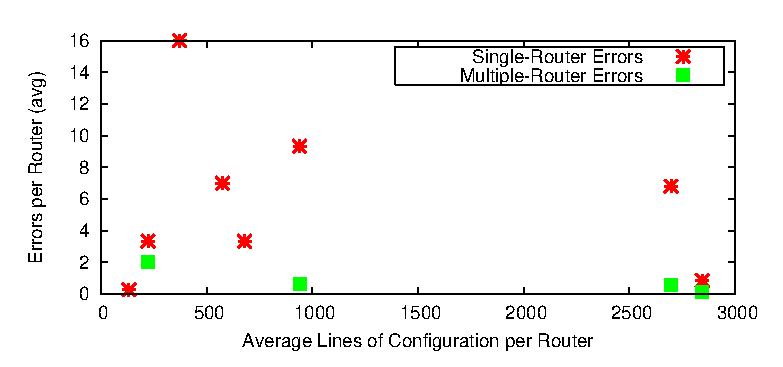
\epsfig{file=rcc/figures/errors_by_loc.eps, width=\linewidth}
%% \caption{Average number of errors per router in an AS vs. the median lines of
%%   configuration for routers in that AS.}
%% \label{fig:errors_by_loc}
%% \end{figure}

%\subsubsection{Effects of Network Size}

%To explore how complexity affects the prevalence of errors in router
%configuration, we examined whether the configuration errors in a network
%are relatively more prevalent in larger networks.  One might expect
%that ASes with larger configuration files, more routers, or more
%sessions might have proportionally more errors. 
%This agrees with our observation
%that errors result from the lack of a systematic process for configuring
%routers, too many levels of indirection, and the fact that the protocol
%itself is so complex that there is little understanding of correct
%configuration in the first place.  These phenomena are true regardless
%of the size or complexity of the AS.
%Figure~\ref{fig:errors_by_loc} shows, for each AS that we had access to
%router configurations, the average number of errors per router in that
%AS vs. the median number of lines of configuration in a router
%configuration in that AS.%\footnote{Median lines of configuration seemed
%to be a better indicator of complexity for BGP configurations than
%average.  Several ASes had many routers with relatively small
%configurations and one or two routers with routers that had
%configurations several orders of magnitude larger.}  
%We consider configuration errors that involve a single router
%(``single-router errors'') separately from errors that involve
%configurations across multiple routers (``multiple-router errors'').


%% \subsection{Prevalence of Anomalies and Errors}

%% Frequency of various types of anomalies.  I think basically we want to
%% say either (1)~we saw this happen in practice (say whether it was once
%% onr ``multiple times''), (2)~we didn't see this, but operators say
%% anecdotally that this type of thing happens frequently.

%% \begin{itemize}
%%         \item whether we tested it (most of these should be "yes")
%%         \item whether it occurred in the configs we saw
%% \begin{itemize}
%%                 \item if so, did it occur multiple times (\ie, in different
%%                   configs for the same AS, in configs in multiple ASes,
%%                   etc.)
%%                 \item if not, whether it occurs "anecdotally" (\ie, does
%%                   Avi Freedman or Randy Bush, etc., say it happens, or has
%%                   the problem been discussed on nanog, been in popular
%%                   press, etc.)
%% \end{itemize}
%%         \item whether the problem should be fixed by:
%% \begin{itemize}
%%                 \item config language fix
%%                 \item protocol fix
%%                 \item decision process fix
%%                 (or some combination)
%% \end{itemize}
%% \end{itemize}




